\documentclass[a4paper,12pt]{article}
\usepackage[UTF8]{ctex}
\usepackage{fullpage}  % leaves 1 inch margins all round
\usepackage{iftex}
\ifPDFTeX
  \usepackage[T1]{fontenc} % modern encoding (more characters available)
  \usepackage{mathptmx} % times in text and mathematics
  \usepackage[scaled]{helvet} % helvetica for sanserif, scaled 95% by default
  \usepackage{courier}  % for typewriter text
\else
  \usepackage{fontspec}
  \usepackage{unicode-math}
  \setmainfont{Times New Roman}
  \setsansfont{Arial}
  \setmonofont{Consolas}
  \setmathfont{Cambria Math}
\fi
\usepackage{textcomp} % lots of useful symbols
\usepackage{graphicx}  % inclusion of graphics files
\usepackage{amsmath}
\usepackage{cite}


\begin{document}

\title{How to write a technical project report}
\author{School of Engineering, University of Glasgow}
\date{\today}
 
\maketitle

\begin{abstract}
All reports start with an \emph{abstract}, which contains a summary of the project: its aim, what was done and what was achieved. This document describes the requirements for a project report in the department and gives advice on how to get better marks. It is structured to match a project report as far as possible.
\end{abstract}

%\tableofcontents

\section{Introduction}

\emph{Whew -- I've finished the work, now I only have to write the report.} Sound familar? Many students put off writing until too late and don't leave enough time to make a good job of the report. This is a serious mistake because the report typically accounts for a large fraction of the assessment. Start early -- most people find report-writing difficult. Think about the report throughout your project, keep track of references and collect material to illustrate the report.

\subsection{Mechanical aspects}

The length of the body of the report will be specified in the instructions for the project. Extra material may be provided in appendices but this material should be for reference only: you cannot assume that the reader will study it. In other words, do not put vital points in an appendix.

You will probably think that the report is too short but this is deliberate. Most reports are submitted to busy managers, who do not have time to read lengthy documents. It is important to learn how to pick out the vital points and write a concise report with maximum impact.

Reports should be word-processed and firmly bound. Use A4 paper and a clear typeface such as 12-point Times, number the pages and leave margins of at least 25\,mm all round. Follow this layout (this document breaks some of the rules to keep it compact).
\begin{itemize}
\item
The front cover should show the title of the project with your name(s) and matriculation number(s) and the name of your supervisor(s).
\item
Put the abstract on the next page. It should be about 100--250 words and gives a brief summary of the report including the background and aims of the project, the principal results and conclusions.
\item
The next page should show the table of contents. 
\item
The body of the report should be divided into numbered sections, each starting on a new page. Figures (diagrams, plots or photographs) and tables need captions and should be numbered.
\end{itemize}

\subsection{What goes into the introduction?}

Explain the background to the project and the reasons why your particular piece of work was considered worthwhile. This leads to the \textbf{aims} of the project: what you are trying to achieve. Be specific.


\section{Body of the report}

\subsection{实验协议与基本设置}

本文的实验分为两个阶段。第一阶段为前期探索实验，用于建立初始基线，并考察输入增强与损失函数设计对分割性能的影响。第二阶段为后期主实验，围绕 DRIVE 数据集 \cite{staal2004drive}，在统一的五折交叉验证框架下验证所提出结构改进模块的有效性。由于两个阶段在数据来源、输入形式、数据划分方式和评价指标上存在差异，本文分别进行说明。

前期探索阶段对应前 3 次实验。该阶段基于多数据源样本训练初始分割模型，并考察不同输入增强和损失设计对模型性能的影响。后期主实验从第 4 次实验开始建立统一实验平台。第 4 次实验在 DRIVE 数据集上建立基线设置，第 5 次实验及后续所有结构改进实验均在相同的数据集、预处理流程和五折划分下进行，以保证横向比较的公平性。

\subsubsection{数据集与数据组织}

在前期探索阶段，训练数据来自多个公开视网膜血管分割数据集，包括 STARE \cite{hoover2000locating}、CHASE\_DB1 \cite{fraz2012ensemble} 和 HRF \cite{budai2013robust}。该阶段使用多数据源训练样本建立初始模型，并考察模型在 DRIVE 目标域上的表现。前 3 次实验采用固定数据划分，而未使用交叉验证。这样设置是为了保持与前期对比工作一致，使所得结果能够在相同数据条件下与师兄的实验结果直接比较。根据现有划分文件，训练集和验证集样本数分别为 801 和 90。

在输入构建方面，前期实验采用三通道分离输入。具体来说，原始彩色眼底图像首先被转换为 nnU-Net 可读取的 NIfTI 格式，然后进一步拆分为红、绿、蓝三个独立通道，分别作为模型输入。这种处理方式保留了彩色图像中的光谱信息，使模型能够分别学习不同颜色通道中的血管特征，也为后续分析绿色通道信息和对比度增强策略提供了条件。

后期主实验仅使用 DRIVE 数据集，并采用统一的数据组织方式。与前期阶段不同，后期实验不再使用三通道彩色输入，而是采用经过增强预处理的单通道图像。具体而言，原始眼底图像依次经过灰度化、标准化、自适应直方图均衡化和 gamma 校正，再转换为单通道 NIfTI 文件输入模型。该处理流程参考 PA-Net 的预处理设置 \cite{luo2025panet}，用于增强细小血管和低对比度区域的可分辨性，并减少无关颜色信息的干扰。

后期实验从第 4 次实验开始建立统一协议。第 4 次实验在 DRIVE 数据集上构建了后期主实验的基线；第 5 次实验以及后续所有结构改进实验均沿用同一套数据组织方式、同一套预处理流程和同一份五折划分文件。因此，后续各模型之间的性能差异主要归因于网络结构、损失函数或后处理策略的变化，而不是数据划分差异。

\subsubsection{实现细节与评价指标}

全部实验基于 nnU-Net v2 框架实现 \cite{isensee2021nnunet}。为保证实验比较的可解释性，同一实验阶段内各组实验采用统一训练流程；除特别说明外，不同实验之间仅在输入预处理、网络结构、损失函数或后处理策略上存在差异。本文后续实验的主要改动集中在 nnU-Net 中 U-Net 主体结构及其特征交互方式上，只有少数实验涉及 trainer 层面的损失函数或训练策略调整。前期探索实验采用固定划分，用于验证不同设计的可行性；后期主实验统一在 DRIVE 数据集上采用 2D 配置和五折交叉验证，用于评估各改进模块的实际效果。

在前期阶段，基线模型训练使用标准 nnU-Net 训练器，并统一设置为 150 个 epoch。前 3 次实验分别对应原始输入下的 baseline、加入 CLAHE 的输入增强版本，以及在增强输入基础上结合 Dice 与 Focal Loss 的版本。该阶段的评价脚本输出 IoU (vessel)、mIoU、Recall、Precision、Accuracy、mPA 和 F1-score，因此前期实验结果以这一组指标报告。

在后期主实验中，模型训练统一采用 nnU-Net v2 的 2D 配置。输入 patch size 设为 \(512 \times 512\)，batch size 设为 2，训练轮数统一设为 100。优化器采用 SGD，初始学习率设为 0.001，并结合 Poly 学习率衰减策略完成训练。除特别说明外，不同模型之间保持相同的数据划分和训练计划。第 4 次实验建立了该阶段的基线，第 5 次实验及后续所有改进模型均在这一统一设置下进行比较。

在评估流程上，后期主实验不直接使用单个 fold 的结果作为最终结论，而是对五折验证结果进行统一汇总后再计算指标。每个 fold 分别生成验证集预测结果，随后在完整交叉验证输出上统一评估，以减小单次划分带来的波动，并提高不同模型之间比较的一致性。

后期主实验采用 Sensitivity (SE)、Specificity (SP)、Accuracy (ACC)、AUC、Precision (PR) 和 F1-score 作为评价指标。SE 用于衡量模型对细小血管和弱响应区域的检出能力，SP 和 PR 用于评估模型抑制伪阳性的能力，ACC 反映整体像素分类准确率，F1-score 用于综合评价分割性能。由于当前实验未保存概率图，本文报告的 AUC 基于二值预测结果近似计算。

\subsection{基线与前期探索}

本文以前期基线实验及围绕基线开展的输入增强、损失函数探索作为后续研究的起点。前 3 次有效实验未重新划分数据，而是沿用既有的训练集和验证集名单，以保持与刘师兄实验设置一致，并便于在相同数据条件下进行直接比较。三次实验均以 DRIVE 数据集作为测试集，并采用统一的前期评价指标体系进行比较。

第一次实验采用标准 nnU-Net 基线模型 \cite{isensee2021nnunet}，以建立初始性能参照。结果表明，该模型在固定划分条件下已经能够取得较稳定的整体分割性能，可作为后续探索的起点。

第二次实验在相同训练框架下引入 CLAHE 图像增强，以考察输入增强对血管分割性能的影响。实验结果表明，CLAHE 有助于改善训练初期的收敛过程，但对最终分割性能的提升有限。这说明输入增强能够改善图像表征质量，但难以单独解决细小血管和复杂结构区域的建模问题。

第三次实验在 CLAHE 基础上进一步引入 Focal Loss，以考察损失函数调整对困难像素和类别不平衡问题的作用。结果表明，该设置能够进一步加快训练收敛，但并未带来稳定的性能提升。这说明在当前模型结构下，仅通过损失函数设计仍不足以突破基线表现。

综合前 3 次实验可以看出，输入增强和损失函数调整能够影响模型训练过程和部分指标表现，但这种改动主要作用于输入表征和优化目标，并未改变模型对细小血管、低对比度区域和结构连续性的建模方式。基于这一观察，后续研究将重点从训练层面的调整转向结构层面的改进。

\begin{table}[htbp]
\centering
\caption{前期探索实验结果汇总}
\label{tab:early_experiments}
\begin{tabular}{llllll}
\hline
实验编号 & 方法 & 训练设置 & 收敛情况 & 代表性结果 & 主要观察 \\
\hline
Exp1 & nnU-Net baseline & Dice, 150 epoch & 第69个 epoch 收敛 & F1 = 0.7924 & 建立前期基线 \\
Exp2 & CLAHE + nnU-Net & Dice, 150 epoch & 第60个 epoch 收敛 & F1 = 0.7827 & 改善早期收敛，但最终提升有限 \\
Exp3 & CLAHE + nnU-Net + Focal Loss & Focal Loss, 150 epoch & 第53个 epoch 收敛 & F1 = 0.7802 & 收敛更快，但性能未进一步提升 \\
\hline
\end{tabular}
\end{table}

\subsection{PA-Net 模块迁移}

在完成基线与前期探索之后，本文首先尝试将 PA-Net 中的两个核心模块迁移到 nnU-Net 框架中，即 Lightweight Parallel Transformer (LPT) 和 Adaptive Vascular Feature Fusion Module (AFFM) \cite{luo2025panet}。这一阶段的目的不是直接得到最终模型，而是先考察 PA-Net 的结构思想在当前任务中的适用性，并据此判断后续优化方向。

LPT 被置于网络的 bottleneck 位置，用于增强模型对长程依赖和全局结构信息的建模能力。PA-Net 中的 LPT 将局部特征建模与并行注意力机制结合起来，在保持较低计算开销的同时扩大特征交互范围。对于视网膜血管分割任务，这种设计有助于在高层语义空间中整合更完整的血管走向和拓扑信息，从而减轻细小血管在深层表示中的断裂和缺失。AFFM 用于替代标准的 skip connection 融合方式，以增强不同层级特征之间的交互。与直接拼接不同，AFFM 对多层血管特征进行自适应加权，使浅层细节与深层语义能够更有选择性地参与解码。对于当前任务，这一设计旨在减轻下采样过程中的细节损失，并改善边缘和分叉区域的恢复效果。

从抽象计算形式上看，若将输入特征记为 \(X\)，则 LPT 中的注意力分支可以写为
\[
Q = XW_Q,\qquad K = XW_K,\qquad V = XW_V,
\]
\[
\mathcal{A}(X) = \mathrm{Softmax}\left(\frac{QK^{\top}}{\sqrt{d}}\right)V,
\]
其中 \(d\) 表示特征维度。若进一步将局部分支记为 \(\mathcal{L}(X)\)，则 LPT 的输出可以概括为
\[
Y_{\mathrm{LPT}} = \mathrm{FFN}\big(\mathcal{L}(X) + \mathcal{A}(X)\big) + X.
\]
这一形式说明，LPT 的核心并不只是引入注意力，而是将局部特征提取与全局依赖建模并行结合后再进行融合。对于 AFFM，若将来自三个层级的输入特征分别记为 \(F_1\)、\(F_2\) 和 \(F_3\)，则其融合过程可以简化表示为
\[
Y_{\mathrm{AFFM}} = \sum_{i=1}^{3}\alpha_i \odot F_i,\qquad
[\alpha_1,\alpha_2,\alpha_3] = \mathrm{Softmax}\big(\phi([F_1,F_2,F_3])\big),
\]
其中 \(\phi(\cdot)\) 表示由卷积映射得到的权重生成函数，\(\odot\) 表示逐元素加权。这一表达强调了 AFFM 的本质在于通过自适应权重调节多层级特征在解码阶段的相对贡献。

\begin{figure}[htbp]
\centering
\begin{minipage}{0.4\textwidth}
\centering
\includegraphics[height=0.22\textheight,keepaspectratio]{pic/panet.png}\\
(a) PA-Net 整体结构
\end{minipage}
\hfill
\begin{minipage}{0.2\textwidth}
\centering
\includegraphics[height=0.22\textheight,keepaspectratio]{pic/LPT.png}\\
(b) LPT 模块结构
\end{minipage}
\hfill
\begin{minipage}{0.33\textwidth}
\centering
\includegraphics[height=0.22\textheight,keepaspectratio]{pic/AFFM.png}\\
(c) AFFM 模块结构
\end{minipage}
\caption{PA-Net 及其迁移到 nnU-Net 的两个核心模块。三幅图采用相同高度以便于横向比较。}
\label{fig:panet_triplet}
\end{figure}

本阶段首先采用完整模块迁移的方式，将 LPT 与 AFFM 同时引入 nnU-Net，并与统一协议下的基线模型进行比较，以获得对整体结构效果的初步观察。由于后续实验的主要改动集中在 nnU-Net 中 U-Net 主体结构及其特征交互方式上，这一步为进一步的消融实验和结构增强提供了直接起点。下一节将分别考察 LPT 和 AFFM 的独立作用，以判断性能变化的具体来源。

\subsection{LPT 与 AFFM 的消融}

在完成 PA-Net 模块迁移之后，本文进一步分别考察 LPT 和 AFFM 的独立作用，以判断完整迁移结果中的性能变化主要来自哪个模块。该部分仍沿用后期主实验的统一设置，即在 DRIVE 数据集上采用相同的单通道预处理流程、相同的五折划分文件和相同的训练计划进行比较。与前文一致，本节不根据单个 fold 的结果直接作结论，而是对五折验证结果统一汇总后再计算评价指标。

考虑到 nnU-Net 框架与网络主体结构耦合较强，本节在基线模型之外，进一步构建了完整 PA-Net 迁移、仅引入 LPT 的 LPT Only 以及仅引入 AFFM 的 AFFM Only 三组模型，以保证比较对象与目标结构一致。其中，LPT Only 对应消融 A，表示仅在 bottleneck 处引入 LPT；AFFM Only 对应消融 B，表示仅将解码阶段的特征融合替换为 AFFM。

\begin{table}[htbp]
\centering
\caption{LPT 与 AFFM 消融实验结果对比}
\label{tab:lpt_affm_ablation}
\resizebox{\textwidth}{!}{
\begin{tabular}{lcccccc}
\hline
实验组 & SE & SP & ACC & AUC & PR & F1-score \\
\hline
nnU-Net v2 Baseline & $0.7627 \pm 0.0446$ & $0.9852 \pm 0.0050$ & $0.9659 \pm 0.0045$ & $0.8739 \pm 0.0210$ & $0.8238 \pm 0.0646$ & $0.7891 \pm 0.0320$ \\
PA-Net (Full) & $0.7211 \pm 0.0763$ & $0.9888 \pm 0.0050$ & $0.9659 \pm 0.0059$ & $0.8549 \pm 0.0365$ & $0.8570 \pm 0.0621$ & $0.7782 \pm 0.0464$ \\
LPT Only (消融 A) & $0.7597 \pm 0.0492$ & $0.9864 \pm 0.0041$ & $0.9669 \pm 0.0044$ & $0.8731 \pm 0.0234$ & $0.8361 \pm 0.0546$ & $0.7935 \pm 0.0297$ \\
AFFM Only (消融 B) & $0.7573 \pm 0.0475$ & $0.9868 \pm 0.0039$ & $0.9672 \pm 0.0045$ & $0.8720 \pm 0.0227$ & $0.8400 \pm 0.0517$ & $0.7942 \pm 0.0300$ \\
\hline
\end{tabular}
}
\end{table}

从表 \ref{tab:lpt_affm_ablation} 可以看出，完整 PA-Net 迁移结果并未优于基线，而两组单模块消融结果整体上表现得更为稳定。其中，LPT Only 在基本保持 SE 的同时略微提高了 PR 和 F1-score，说明在 bottleneck 处引入全局信息建模具有一定参考价值；AFFM Only 虽然取得了本组实验中最高的 ACC 和 F1-score，但这一优势主要体现在本节的局部对比中，尚不足以说明 AFFM 可以作为后续实验的主要改进方向。

综合本节结果可以看出，PA-Net 中单个模块的设计思路可以作为参考，但直接将 LPT 与 AFFM 同时迁移到 nnU-Net 中并不能形成更优结构。因此，本节的作用主要是识别完整迁移中可能存在的问题来源，而不是在此阶段直接确定后续主线方案。基于这一观察，后续实验需要继续分别验证模块本身及其与现有训练机制之间的关系。至于各指标之间更细致的比较与原因分析，将在第三章进一步展开。

\subsection{AFFM 与深监督的兼容性验证}

考虑到 AFFM 在 PA-Net 中用于解码阶段的多层特征融合 \cite{luo2025panet}，而 nnU-Net 中的深监督同样作用于解码阶段的多尺度特征 \cite{isensee2021nnunet,lee2015dsn}，本节进一步增加了一组控制实验，以考察两者在当前框架下是否会产生潜在冲突。该部分仍沿用后期主实验的统一设置，即在 DRIVE 数据集上采用相同的单通道预处理流程、相同的五折划分文件和相同的训练计划进行比较。与前文一致，评价结果基于五折验证结果统一汇总后计算。

在 nnU-Net 的默认训练流程中，深监督会在解码器的多个阶段施加辅助分割损失，以强化多尺度特征学习 \cite{isensee2021nnunet,lee2015dsn}。若将主输出损失记为 \(\mathcal{L}_{\mathrm{main}}\)，将第 \(s\) 个辅助输出损失记为 \(\mathcal{L}_{\mathrm{aux}}^{(s)}\)，则总损失可以写为
\[
\mathcal{L} = \mathcal{L}_{\mathrm{main}} + \sum_{s=1}^{S}\lambda_s \mathcal{L}_{\mathrm{aux}}^{(s)},
\]
其中 \(\lambda_s\) 表示各辅助分支的权重。图 \ref{fig:deep_supervision_cn} 进一步示意了深监督在训练阶段如何通过多个辅助分割头共同参与损失计算，而在推理阶段仅保留主输出。考虑到 AFFM 同样作用于解码阶段的多层特征融合 \cite{luo2025panet}，本节进一步在 AFFM Only 的基础上关闭深监督，构造 AFFM w/o DS 模型，以判断前一节观察到的性能变化是否与深监督有关。表 \ref{tab:affm_ds_cn} 给出了 AFFM 在保留和关闭深监督两种设置下的结果对比。

\begin{figure}[htbp]
\centering
\includegraphics[width=0.95\textwidth]{pic/deep_supervision.png}
\caption{nnU-Net 解码器中深监督机制的示意图。训练阶段在多个解码层附加辅助分割头并共同计算加权总损失，而推理阶段仅保留主输出。}
\label{fig:deep_supervision_cn}
\end{figure}

\begin{table}[htbp]
\centering
\caption{AFFM 在有无深监督下的结果对比}
\label{tab:affm_ds_cn}
\resizebox{\textwidth}{!}{
\begin{tabular}{lcccccc}
\hline
实验组 & SE & SP & ACC & AUC & PR & F1-score \\
\hline
AFFM Only (with DS) & $0.7573 \pm 0.0475$ & $0.9868 \pm 0.0039$ & $0.9672 \pm 0.0045$ & $0.8720 \pm 0.0227$ & $0.8400 \pm 0.0517$ & $0.7942 \pm 0.0300$ \\
AFFM w/o DS & $0.7401 \pm 0.0493$ & $0.9880 \pm 0.0038$ & $0.9667 \pm 0.0048$ & $0.8640 \pm 0.0236$ & $0.8490 \pm 0.0534$ & $0.7883 \pm 0.0308$ \\
\hline
\end{tabular}
}
\end{table}

从表 \ref{tab:affm_ds_cn} 可以看出，关闭深监督后，AFFM 模型的 SP 和 PR 略有提高，但 SE、AUC 和 F1-score 均有所下降，说明模型在预测上变得更为保守。也就是说，去除深监督后，模型虽然能够减少部分伪阳性，但对细小血管和弱响应区域的检出能力有所减弱。

综合本节结果可以看出，关闭深监督并不能使 AFFM 获得更好的整体表现，因此仅靠去除深监督还不足以解释前面观察到的性能变化。本节实验的作用主要在于排除“深监督冲突”这一可能因素，并进一步说明 AFFM 在当前框架下的收益并不稳定。但在这一阶段，是否继续保留 AFFM 仍需结合后续结构实验进一步判断。关于这一现象的更细致讨论，将在第三章进一步展开。

\subsection{LPT 中的可变形注意力}

在完成对 AFFM 与深监督关系的控制实验之后，本文将关注点重新放回 LPT 模块本身，并尝试进一步改进其高层特征建模方式。具体而言，本节参考可变形注意力 \cite{zhu2021deformabledetr} 的思路，将 PA-Net 中 LPT 原有的 GAA 形式 \cite{luo2025panet} 替换为可变形注意力，以增强模型对弯曲血管、分叉结构和细小末梢区域的自适应建模能力。该部分仍沿用后期主实验的统一设置，即在 DRIVE 数据集上采用相同的单通道预处理流程、相同的五折划分文件和相同的训练计划进行比较。与前文一致，评价结果基于五折验证结果统一汇总后计算。

与 GAA 中较为规则的固定采样方式不同，可变形注意力通过为参考位置学习若干偏移量，使特征聚合能够更灵活地分布在目标结构周围。若将参考位置记为 \(p\)，第 \(k\) 个采样偏移记为 \(\Delta p_k\)，对应权重记为 \(A_k\)，则其局部聚合过程可以写为
\[
\mathrm{DefAttn}(p) = \sum_{k=1}^{K} A_k \cdot x(p + \Delta p_k),\qquad
\sum_{k=1}^{K} A_k = 1,
\]
其中 \(K\) 表示采样点数。对于视网膜血管分割任务，这意味着采样位置不必局限于固定方向，而可以更贴近弯曲血管、分叉区域和细小末梢的实际走向。图 \ref{fig:deformable_attention_cn} 给出了 GAA 与可变形注意力采样方式的示意对比。其中，4 point 和 8 point 分别表示每个参考位置周围参与特征聚合的采样点数。

\begin{figure}[htbp]
\centering
\includegraphics[width=0.95\textwidth]{pic/Deformable_Attention.png}
\caption{GAA 与可变形注意力采样方式的示意对比。左图表示较为规则的固定采样，右图表示围绕参考位置进行自适应偏移的采样方式。}
\label{fig:deformable_attention_cn}
\end{figure}

在这一阶段，实验首先构建不含 AFFM 的 Deformable LPT（4 point）模型，用于判断可变形注意力替换本身是否有效；随后在相同设置下重新加入 AFFM，以考察在新的 LPT 结构下是否仍有保留 AFFM 的必要；最后再将采样点数由 4 point 扩展到 8 point，以进一步观察采样规模变化对结果的影响。表 \ref{tab:deformable_lpt_cn} 给出了相关实验结果。

\begin{table}[htbp]
\centering
\caption{可变形 LPT 相关实验结果对比}
\label{tab:deformable_lpt_cn}
\resizebox{\textwidth}{!}{
\begin{tabular}{lcccccc}
\hline
实验组 & SE & SP & ACC & AUC & PR & F1-score \\
\hline
LPT Only & $0.7597 \pm 0.0492$ & $0.9864 \pm 0.0041$ & $0.9669 \pm 0.0044$ & $0.8731 \pm 0.0234$ & $0.8361 \pm 0.0546$ & $0.7935 \pm 0.0297$ \\
Deformable LPT (No AFFM, 4 point) & $0.7634 \pm 0.0540$ & $0.9863 \pm 0.0043$ & $0.9672 \pm 0.0044$ & $0.8749 \pm 0.0254$ & $0.8371 \pm 0.0511$ & $0.7958 \pm 0.0275$ \\
Deformable LPT + AFFM & $0.7571 \pm 0.0495$ & $0.9867 \pm 0.0042$ & $0.9670 \pm 0.0044$ & $0.8719 \pm 0.0235$ & $0.8388 \pm 0.0545$ & $0.7933 \pm 0.0301$ \\
Deformable LPT (No AFFM, 8 point) & $0.7573 \pm 0.0506$ & $0.9869 \pm 0.0038$ & $0.9672 \pm 0.0047$ & $0.8721 \pm 0.0241$ & $0.8412 \pm 0.0504$ & $0.7946 \pm 0.0296$ \\
\hline
\end{tabular}
}
\end{table}

从表 \ref{tab:deformable_lpt_cn} 可以看出，在不引入 AFFM 的条件下，将 LPT 替换为可变形注意力后，模型的 SE、AUC 和 F1-score 均较 LPT Only 有所提升，其中 4 point 设置取得了本组实验中最高的 F1-score。这说明在 bottleneck 位置引入更灵活的空间采样机制后，模型对高层血管结构的建模能力有所增强，也说明这一改动比前面围绕 AFFM 的调整更适合作为后续结构优化的继续方向。

在此基础上，本文进一步测试了 Deformable LPT + AFFM。结果表明，在新的 LPT 结构下重新加入 AFFM 并未带来进一步提升，F1-score 反而从 0.7958 降至 0.7933。这说明即使在可变形注意力替换之后，AFFM 仍未表现出稳定的增益。结合这一结果，本文在这一阶段正式不再将 AFFM 保留为后续实验的组成部分，而是转向以不含 AFFM 的 LPT 改进路径作为后续主线。

最后，本文进一步比较了 4 point 和 8 point 两种采样设置。结果显示，8 point 在 PR 上略有提高，但 SE、AUC 和 F1-score 均未超过 4 point 版本，说明更大的采样规模并未带来更优的整体性能。基于这一观察，后续实验优先保留不含 AFFM 的 Deformable LPT（4 point）设置，并在此基础上继续开展后续结构改进。关于这些变化的更细致分析，将在第三章进一步展开。

\subsection{Modulated 与多尺度可变形 LPT}

在确定不含 AFFM 的 Deformable LPT（4 point）可以作为后续改进基线之后，本文继续沿两个方向展开实验。第一，参考调制可变形机制的思想 \cite{zhu2019dcnv2}，在单尺度可变形采样中加入额外的 modulation mask，以进一步抑制无关位置的响应，并增强对关键采样点的选择能力。第二，参考多尺度可变形注意力的思路 \cite{zhu2021deformabledetr}，将 bottleneck 处的采样范围从当前层扩展到 encoder 多层特征，以考察跨层采样和聚合是否能够补充更多高分辨率细节。该部分仍沿用后期主实验的统一设置，即在 DRIVE 数据集上采用相同的单通道预处理流程、相同的五折划分文件和相同的训练计划进行比较。与前文一致，评价结果基于五折验证结果统一汇总后计算。

若以前一节中的单尺度可变形采样为基础，将第 \(k\) 个采样点的 modulation mask 记为 \(m_k\)，则单尺度 modulated deformable 形式可以写为
\[
\mathrm{ModDefAttn}(p) = \sum_{k=1}^{K} m_k A_k \cdot x(p + \Delta p_k),\qquad
m_k = \sigma(g_k(x)),
\]
其中 \(\sigma(\cdot)\) 表示 Sigmoid 函数，\(g_k(\cdot)\) 表示掩码生成映射。图 \ref{fig:modulated_deformable_cn} 给出了单尺度 Modulated Deformable 采样的示意图，其中 modulation mask 用于进一步调节不同采样点在聚合中的贡献。进一步地，若将多尺度输入特征记为 \(\{x_l\}_{l=1}^{L}\)，并记第 \(l\) 层的线性映射为 \(P_l(\cdot)\)，则多尺度 modulated deformable 聚合可概括为
\[
\mathrm{MSModDefAttn}(p) = \sum_{l=1}^{L}\sum_{k=1}^{K} A_{l,k} m_{l,k} \cdot P_l\big(x_l(p_l + \Delta p_{l,k})\big).
\]
这一形式说明，第二步实验的核心不只是增加采样点，而是让 bottleneck 特征以当前层为 query，跨层访问 encoder 各级特征并进行加权聚合。图 \ref{fig:ms_modulated_cn} 则进一步展示了跨层多尺度采样与聚合的整体过程。

\begin{figure}[htbp]
\centering
\includegraphics[width=0.9\textwidth]{pic/Modulated_Deformable_Sampling.png}
\caption{单尺度 Modulated Deformable 采样示意图。查询点通过可变形偏移访问周围采样位置，并利用 modulation mask 对不同采样点的贡献进行进一步调节。}
\label{fig:modulated_deformable_cn}
\end{figure}

\begin{figure}[htbp]
\centering
\includegraphics[width=0.95\textwidth]{pic/MS_modulated_DF.png}
\caption{多尺度 Modulated Deformable 采样示意图。bottleneck 特征作为 query，跨层访问 encoder 多尺度特征，并通过加权聚合形成增强后的 bottleneck 表示。}
\label{fig:ms_modulated_cn}
\end{figure}

基于上述思路，本节首先在不含 AFFM 的前提下构建 Modulated Deformable（4 point）模型，用于考察 modulation mask 对单尺度可变形采样的影响；随后进一步构建 MS-Modulated（4 point）模型，用于验证跨层多尺度采样是否能够在保持可变形采样灵活性的同时引入更多浅层细节。表 \ref{tab:modulated_msdeform_cn} 给出了相关实验结果。

\begin{table}[htbp]
\centering
\caption{Modulated 与多尺度可变形 LPT 实验结果对比}
\label{tab:modulated_msdeform_cn}
\resizebox{\textwidth}{!}{
\begin{tabular}{lcccccc}
\hline
实验组 & SE & SP & ACC & AUC & PR & F1-score \\
\hline
Deformable LPT (No AFFM, 4 point) & $0.7634 \pm 0.0540$ & $0.9863 \pm 0.0043$ & $0.9672 \pm 0.0044$ & $0.8749 \pm 0.0254$ & $0.8371 \pm 0.0511$ & $0.7958 \pm 0.0275$ \\
Deformable LPT (No AFFM, 8 point) & $0.7573 \pm 0.0506$ & $0.9869 \pm 0.0038$ & $0.9672 \pm 0.0047$ & $0.8721 \pm 0.0241$ & $0.8412 \pm 0.0504$ & $0.7946 \pm 0.0296$ \\
Modulated Deformable (4 point) & $0.7660 \pm 0.0511$ & $0.9858 \pm 0.0048$ & $0.9669 \pm 0.0046$ & $0.8759 \pm 0.0241$ & $0.8324 \pm 0.0560$ & $0.7950 \pm 0.0305$ \\
MS-Modulated (4 point) & $0.7582 \pm 0.0509$ & $0.9870 \pm 0.0038$ & $0.9673 \pm 0.0046$ & $0.8726 \pm 0.0242$ & $0.8419 \pm 0.0497$ & $0.7954 \pm 0.0283$ \\
\hline
\end{tabular}
}
\end{table}

从表 \ref{tab:modulated_msdeform_cn} 可以看出，Modulated Deformable（4 point）在 SE 和 AUC 上取得了本组实验中的最高值，说明引入 modulation mask 后，模型在细小血管和弱响应区域上的检出能力有所增强。这表明在单尺度可变形采样中，额外的选择机制确实能够影响采样分布，使模型更倾向于关注与血管连续性相关的位置。

另一方面，MS-Modulated（4 point）并未继续提高 SE，但在 SP、ACC 和 PR 上取得了更好的表现，说明跨层多尺度采样有助于提高模型对背景噪声的抑制能力，并改善整体预测平衡。也就是说，这一步的收益更多体现在不同层级信息的补充和融合上，而不只是单纯增强灵敏度。

综合本节结果可以看出，modulation 与多尺度扩展分别带来了不同方向的性能变化：前者更倾向于提高血管检出能力，后者更倾向于改善整体平衡性。两者都没有显著超过前一节的 Deformable LPT（4 point）在 F1-score 上的表现，但为后续结果分析提供了更加清晰的结构演化线索。关于这些指标差异的进一步讨论，将在第三章展开。

\subsection{MS-Modulated 与 Coordinate Attention}

在完成 Modulated 与多尺度可变形采样实验之后，本文进一步尝试在 MS-Modulated 结构中引入 Coordinate Attention (CA) \cite{hou2021coordatt}，以继续增强模型对细长血管结构和位置信息的建模能力。与一般通道注意力不同，CA 将位置信息编码到通道注意力之中，并分别沿水平和垂直方向聚合特征，从而在保留长程依赖的同时显式保留空间位置信息。对于视网膜血管分割任务，这类设计尤其适合处理细长、连续且具有明显方向性的血管结构。该部分仍沿用后期主实验的统一设置，即在 DRIVE 数据集上采用相同的单通道预处理流程、相同的五折划分文件和相同的训练计划进行比较。与前文一致，评价结果基于五折验证结果统一汇总后计算。

若将输入特征记为 \(X \in \mathbb{R}^{C\times H\times W}\)，则 CA 可以先沿两个空间方向分别进行聚合，得到
\[
z_h(c,h)=\frac{1}{W}\sum_{i=1}^{W}X(c,h,i),\qquad
z_w(c,w)=\frac{1}{H}\sum_{j=1}^{H}X(c,j,w).
\]
经过共享映射和方向相关变换后，可得到两个方向敏感的注意力图 \(a_h\) 和 \(a_w\)，其输出可以概括为
\[
Y_{\mathrm{CA}} = X \odot a_h \odot a_w.
\]
这一形式说明，CA 的作用并不是替代多尺度可变形采样，而是在其基础上进一步强调与血管方向和位置相关的响应区域，从而改善特征表达的空间选择性。图 \ref{fig:ms_ca_cn} 展示了 MS-Modulated 与 CA 结合后的整体结构示意。

\begin{figure}[htbp]
\centering
\includegraphics[width=0.95\textwidth]{pic/MS_CA.png}
\caption{MS-Modulated 与 Coordinate Attention 结合的结构示意图。多尺度可变形采样先完成跨层信息聚合，随后由 Coordinate Attention 在空间方向上进一步重标定特征响应。}
\label{fig:ms_ca_cn}
\end{figure}

基于上述思路，本节将 MS-Modulated（4 point）作为直接对照组，并进一步构建 MS-Modulated + CA 模型，以考察在已有跨层可变形采样基础上引入显式位置注意力后，模型是否能够取得更稳定的综合表现。表 \ref{tab:msmod_ca_cn} 给出了相关实验结果。

\begin{table}[htbp]
\centering
\caption{MS-Modulated 与 MS-Modulated + CA 实验结果对比}
\label{tab:msmod_ca_cn}
\resizebox{\textwidth}{!}{
\begin{tabular}{lcccccc}
\hline
实验组 & SE & SP & ACC & AUC & PR & F1-score \\
\hline
nnU-Net v2 (Baseline) & $0.7627$ & $0.9852$ & $0.9659$ & $0.8739$ & $0.8238$ & $0.7891$ \\
Modulated (单尺度, 4 point) & $0.7660$ & $0.9858$ & $0.9669$ & $0.8759$ & $0.8324$ & $0.7950$ \\
MS-Modulated (4 point) & $0.7582$ & $0.9870$ & $0.9673$ & $0.8726$ & $0.8419$ & $0.7954$ \\
MS-Modulated + CA & $0.7697$ & $0.9857$ & $0.9673$ & $0.8777$ & $0.8324$ & $0.7973$ \\
\hline
\end{tabular}
}
\end{table}

从表 \ref{tab:msmod_ca_cn} 可以看出，在 MS-Modulated 的基础上引入 CA 后，模型在 SE、AUC 和 F1-score 上进一步提升，其中 SE 达到 0.7697，AUC 达到 0.8777，F1-score 提升到 0.7973。这说明在已有跨层可变形采样的基础上，进一步引入显式位置注意力后，模型对于细小血管和弱响应区域的检出能力得到了增强，同时整体分割质量也有所改善。

与前一节相比，MS-Modulated 更偏向于提升 SP、ACC 和 PR，而加入 CA 后，模型又在 SE、AUC 和 F1-score 上取得了更好的结果。这说明 CA 的主要作用并不只是继续抑制伪阳性，而是帮助模型在保持整体稳定性的同时，更有效地恢复细长血管结构。换言之，多尺度可变形采样负责增强跨层信息交互，而 CA 进一步提升了这些信息在空间维度上的选择性表达。

综合本节结果可以看出，MS-Modulated + CA 在这一阶段取得了最好的综合表现，因此它成为后续结构改进的重要过渡结果。与此同时，这一阶段也说明，在可变形采样已经能够提供灵活取样能力的前提下，显式保留方向和位置信息仍然能够带来额外收益。关于这些结果在不同指标上的进一步比较与讨论，将在第三章展开。

\subsection{MS-DSConv 与 CA}

在得到 MS-Modulated + CA 之后，本文进一步关注到一个新的问题：虽然多尺度可变形采样与 Coordinate Attention 已经增强了跨层信息交互和空间位置选择能力，但当前采样方式本质上仍更接近离散点式建模，能够找到关键位置，却未必能够充分描述血管这种细长、连续、弯曲的几何形态。基于这一观察，后续实验进一步引入动态蛇形卷积（Dynamic Snake Convolution, DSConv）\cite{qi2023dsc}，希望让采样点之间形成连续的轨迹约束，从而更贴合视网膜血管的真实走向。需要说明的是，这一步并不是将整个网络中的普通卷积全部替换为蛇形卷积，而是将其用于 bottleneck 处 LPT 模块中的多尺度采样分支，用来替代前一阶段 MS-Modulated 中的离散点式跨层可变形采样。该部分仍沿用后期主实验的统一设置，即在 DRIVE 数据集上采用相同的单通道预处理流程、相同的五折划分文件和相同的训练计划进行比较。与前文一致，评价结果基于五折验证结果统一汇总后计算。

与前面可变形注意力中各采样点相对独立的形式不同，动态蛇形卷积的关键在于让后续采样位置依赖前面位置的偏移结果。若将第 \(k\) 个采样点的纵向增量记为 \(\delta y_k\)，横向基础步长记为 \(\Delta x_k\)，则蛇形轨迹上的采样位置可以概括为
\[
\tilde{p}_k = p + \left(\Delta x_k,\; \sum_{t=1}^{k}\delta y_t\right).
\]
在多尺度场景下，若进一步将第 \(l\) 个尺度上的聚合写为
\[
\mathrm{MSDSConv}(p) = \sum_{l=1}^{L}\sum_{k=1}^{K} A_{l,k} m_{l,k}\cdot P_l\big(x_l(\tilde{p}_{l,k})\big),
\]
则其与前面多尺度 modulated deformable 的主要区别在于：采样点不再被看作彼此独立的离散位置，而是沿着一条连续展开的轨迹进行聚合。这种设计更适合描述血管的弯曲性、连通性和拓扑连续性，也更适合作为 LPT 在 bottleneck 阶段建模高层血管结构的一种增强方式。图 \ref{fig:msds_ca_cn} 展示了多尺度动态蛇形卷积与 CA 结合后的整体结构示意。

\begin{figure}[htbp]
\centering
\includegraphics[width=0.95\textwidth]{pic/MSDS.png}
\caption{MS-DSConv 与 Coordinate Attention 结合的结构示意图。多尺度采样分支中的采样点沿连续蛇形轨迹展开，在完成跨层加权聚合后，再由 Coordinate Attention 对空间响应进行进一步重标定。}
\label{fig:msds_ca_cn}
\end{figure}

基于上述思路，本节将 MS-Modulated + CA 作为直接对照组，并进一步构建 MS-DSConv + CA 模型，以考察在已有多尺度采样和空间注意力基础上引入连续几何轨迹建模后，模型是否能够进一步提升细小血管的恢复能力和整体结构完整性。表 \ref{tab:msdsconv_ca_cn} 给出了相关实验结果。

\begin{table}[htbp]
\centering
\caption{MS-Modulated + CA 与 MS-DSConv + CA 实验结果对比}
\label{tab:msdsconv_ca_cn}
\resizebox{\textwidth}{!}{
\begin{tabular}{lcccccc}
\hline
实验组 & SE & SP & ACC & AUC & PR & F1-score \\
\hline
nnU-Net v2 (Baseline) & $0.7627$ & $0.9852$ & $0.9659$ & $0.8739$ & $0.8238$ & $0.7891$ \\
MS-Modulated (4 point) & $0.7582$ & $0.9870$ & $0.9673$ & $0.8726$ & $0.8419$ & $0.7954$ \\
MS-Modulated + CA & $0.7697$ & $0.9857$ & $0.9673$ & $0.8777$ & $0.8324$ & $0.7973$ \\
MS-DSConv + CA & $0.8083$ & $0.9815$ & $0.9666$ & $0.8949$ & $0.7997$ & $0.8020$ \\
\hline
\end{tabular}
}
\end{table}

从表 \ref{tab:msdsconv_ca_cn} 可以看出，在 MS-Modulated + CA 的基础上进一步引入动态蛇形卷积后，模型在 SE、AUC 和 F1-score 上取得了明显提升，其中 SE 提升到 0.8083，AUC 提升到 0.8949，F1-score 提升到 0.8020。这说明当采样机制从“独立点式选择”进一步过渡到“连续轨迹式建模”后，模型对细小血管、断裂区域以及连续拓扑结构的恢复能力得到了明显增强。

与此同时，MS-DSConv + CA 的 SP 和 PR 相比前一节略有下降，其中 PR 为 0.7997，低于 0.8，说明这种更强调几何连续性的建模方式会使模型倾向于检出更多潜在血管像素，从而在一定程度上增加伪阳性和小噪声区域。但从整体指标看，这种变化换来了更强的细小血管检出能力和更高的综合分割性能，也更符合视网膜血管分割中对结构连续性的核心需求。

综合本节结果可以看出，MS-DSConv + CA 在这一阶段取得了新的最好结果，但其较低的 PR 也说明结果中仍存在一定误检区域。与前面各步主要围绕“采样位置选择”和“跨层信息融合”不同，这一步进一步强化了对血管几何连续性的建模，因此成为后续继续优化拓扑一致性和结构完整性的关键基础。基于这一观察，下一步实验进一步引入了基于面积阈值的小连通域后处理，以在尽量保持细小血管检出能力的同时提升结果的干净程度和稳定性。

\subsection{小连通域后处理}

在得到 MS-DSConv + CA 之后，本文进一步注意到：虽然该模型在 SE、AUC 和 F1-score 上已经取得了新的最好结果，但其 PR 仍低于 0.8，这说明预测结果中仍存在一定数量的小噪声连通域和伪阳性区域。基于这一现象，后续实验进一步加入了基于面积阈值的小连通域后处理，尝试在保留主要血管结构的同时去除面积过小的孤立预测区域。该步骤不改变主干网络结构，而是在模型输出的二值分割图上执行简单的区域筛除规则。

若将预测结果中的一个连通域记为 \(C_i\)，其像素面积记为 \(|C_i|\)，面积阈值记为 \(X\)，则后处理规则可以简化表示为
\[
\hat{Y}_{\mathrm{post}}(C_i)=
\begin{cases}
1, & |C_i| \ge X,\\
0, & |C_i| < X.
\end{cases}
\]
其中，\(X=0\) 表示不做后处理；当 \(X\) 增大时，更多面积较小的连通域会被移除。图 \ref{fig:postprocess_threshold_cn} 展示了不同阈值下主要指标的变化趋势，其中可以更直观地看到 SE 与 PR 之间的权衡关系以及 \(X=20\) 附近的最佳 F1 平衡点。表 \ref{tab:postprocess_cn} 给出了在不同阈值下的实验结果。

\begin{figure}[htbp]
\centering
\includegraphics[width=0.9\textwidth]{pic/Postprocess_Threshold_Metrics_dual_axis.png}
\caption{后处理面积阈值对主要指标的影响。左侧纵轴表示 SE、PR 和 F1-score，右侧纵轴表示 SP，用于更清楚地展示不同量级指标随阈值变化的趋势。}
\label{fig:postprocess_threshold_cn}
\end{figure}

\begin{table}[htbp]
\centering
\caption{MS-DSConv + CA 在不同后处理阈值下的结果对比}
\label{tab:postprocess_cn}
\resizebox{\textwidth}{!}{
\begin{tabular}{lcccccc}
\hline
实验组 & SE & SP & ACC & AUC & PR & F1-score \\
\hline
MS-DSConv + CA ($X=0$) & $0.8083$ & $0.9815$ & $0.9666$ & $0.8949$ & $0.7997$ & $0.8020$ \\
MS-DSConv + CA ($X=20$) & $0.8059$ & $0.9819$ & $0.9668$ & $0.8939$ & $0.8035$ & $0.8027$ \\
MS-DSConv + CA ($X=30$) & $0.8046$ & $0.9821$ & $0.9669$ & $0.8933$ & $0.8048$ & $0.8026$ \\
MS-DSConv + CA ($X=90$) & $0.7995$ & $0.9827$ & $0.9670$ & $0.8911$ & $0.8089$ & $0.8021$ \\
\hline
\end{tabular}
}
\end{table}

从表 \ref{tab:postprocess_cn} 可以看出，在不做后处理时，即 \(X=0\)，模型已经具有最强的血管检出能力，其中 SE 为 0.8083，AUC 为 0.8949，F1-score 为 0.8020。但与此同时，PR 仅为 0.7997，说明结果中仍保留了一部分误检区域。随着阈值从 0 增加到 20、30 和 90，SP、PR 和 ACC 逐渐上升，而 SE 和 AUC 逐渐下降，这表明后处理确实能够清理掉部分小噪声区域，但也会不可避免地删除一部分真实的细小血管。

进一步比较可见，\(X=20\) 时 F1-score 达到最高的 0.8027，说明这一阈值在去除伪阳性和保留细小血管之间取得了更好的平衡；\(X=30\) 时 PR 和 SP 更高，说明结果更保守、更干净；而当阈值增大到 \(X=90\) 时，虽然 PR 提升到 0.8089，但 SE 已下降到 0.7995，说明阈值过大时会误删一部分真实血管，尤其是面积较小的末梢结构。

综合本节结果可以看出，后处理是有必要的，但阈值需要控制在适中范围内。对于当前实验，适度的小连通域筛除能够在不显著破坏血管连通性的前提下提高预测结果的干净程度和稳定性，因此可以作为网络输出后的有效补充步骤。关于不同阈值下的进一步比较与最终选择，将在第三章展开。

\subsection{clDice 损失探索}

在完成 MS-DSConv + CA 及其后处理实验之后，本文进一步尝试从损失函数层面增强模型对血管拓扑连续性的约束。具体而言，在保持 MS-DSConv + CA 主体结构不变的前提下，本文在原有基础损失之上额外加入 clDice 损失，用于强化对细长结构骨架一致性和连通性的建模。根据当前实现，clDice 仅作用于最高分辨率输出分支，并以附加项的形式与原有损失共同优化，其中其权重设置为 0.3。

为与前一节保持一致，本文同样在不同面积阈值 \(X\) 下评估加入 clDice 之后的结果。表 \ref{tab:cldice_cn} 给出了相关实验结果。

\begin{table}[htbp]
\centering
\caption{加入 clDice 后在不同后处理阈值下的结果对比}
\label{tab:cldice_cn}
\resizebox{\textwidth}{!}{
\begin{tabular}{lcccccc}
\hline
实验组 & SE & SP & ACC & AUC & PR & F1-score \\
\hline
MS-DSConv + CA + clDice ($X=0$) & $0.8110 \pm 0.0477$ & $0.9806 \pm 0.0052$ & $0.9661 \pm 0.0041$ & $0.8958 \pm 0.0220$ & $0.7944 \pm 0.0500$ & $0.8003 \pm 0.0243$ \\
MS-DSConv + CA + clDice ($X=20$) & $0.8079 \pm 0.0484$ & $0.9810 \pm 0.0052$ & $0.9663 \pm 0.0041$ & $0.8945 \pm 0.0223$ & $0.7976 \pm 0.0500$ & $0.8004 \pm 0.0244$ \\
MS-DSConv + CA + clDice ($X=30$) & $0.8061 \pm 0.0486$ & $0.9812 \pm 0.0052$ & $0.9663 \pm 0.0041$ & $0.8937 \pm 0.0224$ & $0.7990 \pm 0.0499$ & $0.8002 \pm 0.0245$ \\
MS-DSConv + CA + clDice ($X=90$) & $0.8002 \pm 0.0498$ & $0.9817 \pm 0.0051$ & $0.9663 \pm 0.0042$ & $0.8910 \pm 0.0230$ & $0.8025 \pm 0.0496$ & $0.7989 \pm 0.0243$ \\
\hline
\end{tabular}
}
\end{table}

从表 \ref{tab:cldice_cn} 可以看出，加入 clDice 后，模型在不同阈值下的 SE 和 AUC 普遍略有提升。例如，在 \(X=0\) 时，SE 提升到 0.8110，AUC 提升到 0.8958；在 \(X=20\) 时，SE 为 0.8079，AUC 为 0.8945。这说明 clDice 作为面向细长结构拓扑一致性的附加损失，确实对血管检出能力和结构连续性建模具有一定积极作用。

然而，与前一节不加入 clDice 的结果相比，这一改动并未带来更好的综合性能。以当前最优的后处理阈值 \(X=20\) 为例，加入 clDice 后的 F1-score 为 0.8004，低于不加入 clDice 时的 0.8027；PR 也从 0.8035 下降到 0.7976。这说明 clDice 虽然增强了模型对细小血管和拓扑结构的敏感性，但同时也带来了更多伪阳性区域，使得整体平衡性反而下降。

进一步比较还可以看出，随着后处理阈值增大，加入 clDice 后的趋势与前一节基本一致：SE 和 AUC 逐渐下降，而 SP 和 PR 逐渐上升。这说明后处理与 clDice 并不存在方向上的冲突，但在当前网络结构和损失权重配置下，clDice 仍未能超过不加入 clDice 时的最好结果。

综合本节结果可以看出，clDice 是一次与任务目标高度相关且合理的探索，但在当前实验条件下并未带来稳定的综合性能提升，因此本文未将其保留为最终方案。关于其与结构改进之间关系的进一步讨论，将在第三章展开。

\subsection{本章小结}

本章围绕 nnU-Net 框架中的结构改进与训练策略调整，系统梳理了从 PA-Net 模块迁移到后续多阶段优化的实验演进过程。前期结果表明，直接迁移完整 PA-Net 结构并不能形成更优方案，因此后续研究逐步将重点集中到 LPT 路线，并围绕可变形采样、多尺度跨层信息交互、Coordinate Attention 以及动态蛇形卷积等方向持续改进。实验结果显示，MS-DSConv + CA 在本章范围内取得了最优的综合表现，而后处理进一步改善了结果的干净程度与稳定性。相比之下，AFFM 和 clDice 虽然都具有一定探索价值，但在当前实验条件下未能形成更优的最终方案。基于这些观察，下一章将对各阶段模型的性能差异及其原因进行集中分析与讨论。

\subsection{Structure and sections}

The structure of the report and the titles of sections depend on the nature of the project. Here are suggestions for two extreme types, which can be adjusted to suit your report.

\subsubsection{Research projects}

Here you are given a starting point and a general direction: your aim is to discover something new. The report would probably be divided into sections with familiar titles.
\begin{itemize}
\item
\textbf{Theory} -- 
Explain essential background theory that is vital to understand your report. Select and present the material to show its relevance to the project and demonstrate your understanding. Do not repeat standard material from textbooks, which is a waste of space; give a reference instead. 
%Detailed mathematical derivations should be left to an appendix.

\item
\textbf{Experimental Techniques} --
Give an account of your experimental (or numerical) techniques. Emphasise details that would be necessary to continue the work or to compare your results with those of other experimenters. Aim to include what you would have liked to know at the start of your project.

\item
\textbf{Results} --
Describe these at an appropriate level of detail to support your conclusions. Lengthy tables should be left to an appendix or supplied on a CD. Avoid unnecessary detail: describe preliminary experiments briefly if at all, unless they illustrate some important point.
\end{itemize}


\subsubsection{Design, build and test projects}

Here the goal is specified, more or less precisely: your job is to work out how to get there. The titles of the sections are less standardised but here is a possible approach.
\begin{itemize}
\item
\textbf{Specification} --
Typically you are given only a vague description of the functions required and must first develop this into a firm specification against which your final product will be judged.
\item
\textbf{Possible strategies} --
Evaluate \emph{briefly} the possible approaches that you considered 
%for the overall design 
and explain why you selected one of these. 
Avoid excessive detail of discarded possibilities.
\item
\textbf{Implementation} --
Describe the final product. Concentrate on key features that required advanced design and skim over well-known aspects. Mention useful points that might help future students, such as tricky sections of data sheets.

\textbf{Software} is tricky. Often the best approach is to describe the high-level structure in the main text (a diagram of a state machine for example) and pick out any special features of the program. A complete listing should be included as an appendix or on a CD.
\item
\textbf{Testing} --
This is equivalent to the `Results' section of a research project. 
%and the same comments apply.
\end{itemize}


\subsection{Style of writing}

One of the most difficult aspects of writing is to judge the level and background of your readers. Typically the report will be assessed by your first supervisor, who is an expert on the topic, and your second supervisor, who is not. You should therefore assume that the reader is a \emph{well-educated, graduate engineer} but not an expert on the subject of the project. Assume that he or she is familiar with the general concepts taught in courses up to level 3 but not with the details of specialised courses at higher levels.

It is also difficult to appreciate that most readers are not interested in the nitty-gritty detail. They want to know \emph{what} you did and \emph{why} you did it that way but they don't want a step-by-step account of \emph{how} you did it. Your watchword should therefore be:
\begin{center}
\textbf{SUMMARISE!}
\end{center}
Of course some people need the details -- a person continuing work on the project requires precise experimental methods, for instance. Such material may be better in an appendix. The same is true for computer programs and schematics of complicated circuits. Design-and-build projects may need a User's Manual, which should be included as an appendix. 

A report is a formal document and should be written in appropriate language. Numerous books offer advice on writing reports and a selection \cite{jve05,mkm06,dfb09,tmy05} is listed in the references at the end. Here are a few tips.
\begin{itemize}
\item
Reports should be written in correct English. Break text into paragraphs, keep sentences to a reasonable length and insert appropriate punctuation. Use a spell-checker and a grammar-checker if desired but neither is a substitute for careful reading. 
\item
A report is not a story. 
%Write `The transistor exploded', not `I blew up the transistor'. Similarly, 
Write `The voltage was measured' rather than `I measured the voltage'. This document contains instructions and therefore uses a different style.
\item
Define all abbreviations when they are first used: `The accelerometer uses a serial peripheral interface (SPI)'. Provide a list of abbreviations if you use a large number of them.
\item
Don't write material that you don't understand. It will be obvious to the reader.
\end{itemize}
The quality of English is assessed as part of the report. Foreign students may feel this to be a burden but part of their education in this country is to learn to work effectively in an English-speaking environment. 

\subsection{Precision}

An engineering report must be precise. This applies both to the language and to numerical values. For example, the words \emph{precision} and \emph{accuracy} are often used interchangably in non-technical discussion but the distinction between them is vital in engineering.

Quote numerical results to an appropriate number of significant figures. For example, it is pointless to claim that a length was 12.345\,mm if it was measured with a pocket ruler. Don't simply write down all the digits displayed on your calculator. 

Analyse the uncertainties in your results to increase the impact of your results. Please avoid horrors like this:
\begin{quote}
The gain was quite accurate.
\end{quote}
The sentence is meaningless and the reader will doubt whether you have any idea of the accuracy. Contrast this sentence:
\begin{quote}
The accuracy of the gain was estimated to be $\pm 2\%$, limited by the tolerance of the resistors. A detailed analysis is given in Appendix C.
\end{quote}
This is informative and convinces the reader that you have a full understanding.

\subsection{Figures and tables}

\begin{figure}
\centering
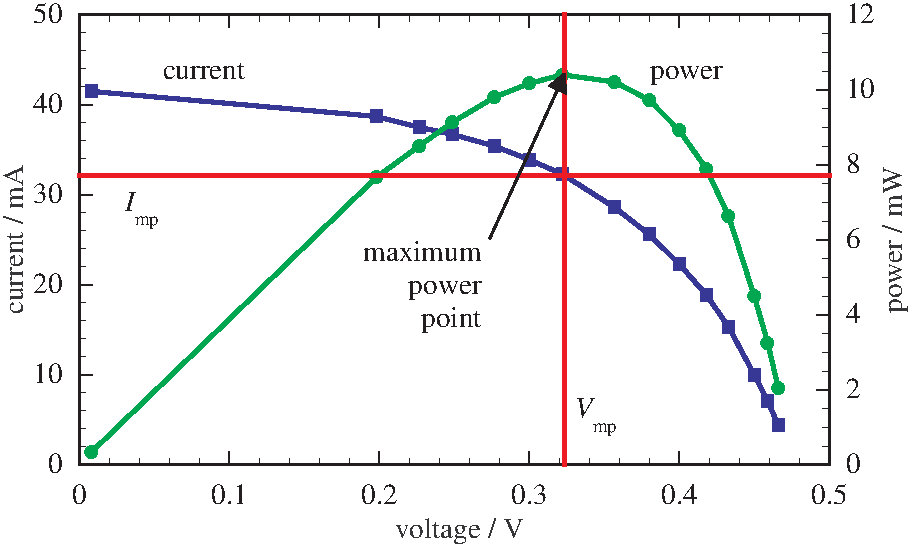
\includegraphics[scale=0.72]{solarcell}
\caption{Current and power as a function of voltage delivered by a single photovoltaic cell under illumination from a 150\,W metal halide floodlamp, showing the maximum power point.}
\label{solar cell fig}
\end{figure}

Figures and tables must have informative captions and be numbered as in Figure~\ref{solar cell fig}. Axes of graphs should have scales, titles and units, otherwise the plot is meaningless. All text must be legible, roughly the same size as the main text. Be warned that plots from Excel need extensive editing to bring them up to an acceptable standard. Oscilloscope screenshots can make good illustrations and are simple to capture on modern equipment.

Tables must have appropriate headings with units. Avoid lengthy tables: consider whether a graph would be clearer or the data would be better on a CD.

\subsection{References}

No project is done in isolation. A research project builds on the results of previous workers; a design-and-build project depends on the properties of the components available. You therefore draw on published documents during your project and must provide \emph{references} to these sources in your report. References are cited (a)~to give due credit to the originator and (b)~to guide a reader who wants more detailed information. You should give a reference wherever it is required for either of these purposes. Properly referenced material from many sources is a sign of a good project report. 
%This section explains how to present such references and how you will be penalised if you fail to do this. The mark for the report include an element for references to reflect their importance.

References must be cited with sequential numbers in square brackets where they are used in the text, not just listed at the end of the report. Typical usage is `Fitzmaurice and Hand \cite{gmf87} showed that\dots' or `The median is an appropriate estimator for this signal \cite{gmf87}'.

Avoid direct quotations from references in general; make it absolutely clear that the text is a quotation if this is unavoidable. An illustration, such as a diagram from a data sheet, is another type of quotation and must be referenced, typically in the figure caption. This is perfectly acceptable: do not waste time redrawing diagrams.

\subsubsection{Plagiarism}

If you copy from another person's work (project report, book, journal, web page or any other document) without acknowledging the source, you are guilty of \emph{plagiarism}. This is a disciplinary offence and the University has procedures for handling it. The failure to acknowledge a source is considered as plagiarism even if there was no deliberate intention to cheat. 

Avoid any risk of plagiarism by providing a reference for all sources that you use. Read the advice offered by the University Library and consult your supervisor if you are in any doubt. The University's \emph{Plagiarism Statement} is reproduced in Appendix \ref{plagiarism sect}.

\subsubsection{List of references}

All reports must have a section entitled `References' after the main text but before any appendices. This comprises a list of references, numbered to match the citations in the text. Each reference requires the following information and the cited references provide examples.
\begin{itemize}
\item
\textbf{Journal paper}: 
author(s), title of paper, name of journal, volume number, first page, last page and year \cite{gmf87}. 
Many journals now use article numbers instead of page numbers.
\item
\textbf{Book}: 
author(s), title, edition, publisher and year of publication \cite{jve05}.
Include the number of the chapter or page(s) if you refer to only a small part of the book.
\item
\textbf{Data sheet}: 
company, title, edition and date \cite{s08qg}. 
Application notes, technical reports and similar documents should be cited in the same way.
\item
\textbf{Web page}: 
author(s) or organisation, title, full URL and date of viewing \cite{mac09}. See below.
\end{itemize}
%The general rule is that 
The reader must be able to find the document without searching for further information.

\subsubsection{References from the Web}

The World Wide Web is a wonderful resource because it is so easy to search. It is therefore tempting to use web pages as references. \emph{Proceed with caution} because the accuracy of many web sites cannot be verified. This is particularly true for anonymous sites such as Wikipedia. Use them only as a starting point: good pages provide references to more authoritative sources.

Reports whose references are all or mainly from the web, especially from anonymous sites, will be penalised.


\section{结果分析与讨论}

本章将在第二章实验演进的基础上，对关键模型的性能变化进行集中比较与讨论。与第二章不同，本章不再按照时间顺序重复叙述每一步实验，而是从整体结果、关键指标权衡、结构演化路径以及后处理与损失函数探索四个角度，对本研究中较为重要的模型进行归纳分析。考虑到当前 AUC 是在二值预测结果上进行近似计算，本章在讨论时将更加重视 SE、PR、SP 与 F1-score 所反映的实际分割表现。

\subsection{整体结果对比}

为便于建立统一参照，表 \ref{tab:chapter3_overall_cn} 汇总了本研究中具有代表性的阶段性结果。该表既包含直接迁移 PA-Net 的早期对照，也包含后续沿着 LPT 主线逐步演化得到的关键模型，从而能够更清楚地展示本研究性能变化的整体轨迹。

\begin{table}[htbp]
\centering
\caption{第三章代表性模型整体结果对比}
\label{tab:chapter3_overall_cn}
\resizebox{\textwidth}{!}{
\begin{tabular}{lcccccc}
\hline
模型 & SE & SP & ACC & AUC & PR & F1-score \\
\hline
nnU-Net v2 Baseline & $0.7627$ & $0.9852$ & $0.9659$ & $0.8739$ & $0.8238$ & $0.7891$ \\
PA-Net (Full) & $0.7211$ & $0.9888$ & $0.9659$ & $0.8549$ & $0.8570$ & $0.7782$ \\
Deformable LPT (No AFFM, 4 point) & $0.7634$ & $0.9863$ & $0.9672$ & $0.8749$ & $0.8371$ & $0.7958$ \\
MS-Modulated (4 point) & $0.7582$ & $0.9870$ & $0.9673$ & $0.8726$ & $0.8419$ & $0.7954$ \\
MS-Modulated + CA & $0.7697$ & $0.9857$ & $0.9673$ & $0.8777$ & $0.8324$ & $0.7973$ \\
MS-DSConv + CA & $0.8083$ & $0.9815$ & $0.9666$ & $0.8949$ & $0.7997$ & $0.8020$ \\
MS-DSConv + CA ($X=20$) & $0.8059$ & $0.9819$ & $0.9668$ & $0.8939$ & $0.8035$ & $0.8027$ \\
\hline
\end{tabular}}
\end{table}

从表 \ref{tab:chapter3_overall_cn} 可以看出，直接迁移完整 PA-Net 并未形成优于 nnU-Net v2 baseline 的结果。虽然 PA-Net (Full) 的 PR 达到 0.8570，说明其输出相对保守、误检较少，但其 SE 仅为 0.7211，显著低于 baseline 的 0.7627，最终 F1-score 也下降到 0.7782。换言之，完整迁移后的模型更倾向于保留高置信度血管区域，却牺牲了大量细小血管和弱响应区域的检出能力。这一现象说明，模块设计本身并非无效，但直接移植到 nnU-Net 框架中并不能自动获得更优结果。

与之相比，后续沿 LPT 路线展开的改进表现出更稳定的提升趋势。Deformable LPT (No AFFM, 4 point) 已将 F1-score 提升到 0.7958，表明在 bottleneck 处引入更灵活的采样方式确实能够改善高层血管结构建模。随后，MS-Modulated 虽未继续提高 SE，但在 SP、ACC 与 PR 上更具优势，体现出更好的整体平衡；在其基础上加入 CA 后，SE、AUC 与 F1-score 再次上升，说明显式方向与位置信息对细长血管恢复仍然具有正向作用。进一步引入 MS-DSConv 后，模型的 SE 提升到 0.8083，F1-score 提升到 0.8020，表明连续几何轨迹建模在本任务中具有更强的结构适配性。

最终结果出现在 MS-DSConv + CA 配合面积阈值为 \(X=20\) 的后处理设置下，其 F1-score 达到 0.8027，相比 baseline 的 0.7891 提升了 0.0136。需要指出的是，这一提升并不是由后处理单独带来的，而是以前面结构改进所建立的较强血管检出能力为前提，再通过轻量的输出筛除机制修正低 PR 问题后形成的。因此，本研究最终保留的方案并不是某一个单独模块“突然奏效”，而是多轮结构优化与结果筛选共同作用的结果。

\subsection{关键指标权衡分析}

从视网膜血管分割任务的需求出发，SE 主要反映细小血管和弱响应区域的检出能力，PR 与 SP 更能体现模型对伪阳性的抑制能力，而 F1-score 则代表二者之间的综合平衡。因而，对各模型的判断不能只依据“某个指标更高”，而应关注不同结构改动究竟把模型推向了更敏感还是更保守的方向。本节的图示主要聚焦于后期主线模型，即 baseline 之后沿 LPT 路线逐步演化并最终保留的结构。

\begin{figure}[htbp]
\centering
\begin{minipage}{0.32\textwidth}
\centering
\includegraphics[width=\textwidth]{pic/Comparison_of_SE_DF.png}\\
(a) SE 对比
\end{minipage}
\hfill
\begin{minipage}{0.32\textwidth}
\centering
\includegraphics[width=\textwidth]{pic/Comparison_of_F1_DF.png}\\
(b) F1-score 对比
\end{minipage}
\hfill
\begin{minipage}{0.32\textwidth}
\centering
\includegraphics[width=\textwidth]{pic/Comparison_of_AUC_DF.png}\\
(c) AUC 对比
\end{minipage}
\caption{后期主线代表性模型在 SE、F1-score 与 AUC 上的变化趋势。}
\label{fig:chapter3_metric_triplet_cn}
\end{figure}

\begin{figure}[htbp]
\centering
\includegraphics[width=0.82\textwidth]{pic/Performance_Balance_Comparison.png}
\caption{后期主线代表性模型在灵敏度与精确率之间的性能平衡对比。}
\label{fig:chapter3_balance_cn}
\end{figure}

结合图 \ref{fig:chapter3_metric_triplet_cn} 与图 \ref{fig:chapter3_balance_cn} 可以看出，Deformable LPT 与 Modulated Deformable 更倾向于提升模型对细小血管的检出能力。其中，Deformable LPT 在保持 PR 基本稳定的同时，将 F1-score 提升到 0.7958；Modulated Deformable 则进一步把 SE 提升到 0.7660，并取得本阶段较高的 AUC，说明 modulation mask 的引入使模型更加关注潜在血管响应区域。不过，这类改动的共同特点是更偏向“提高敏感度”，而不是显著改善误检抑制能力。

MS-Modulated 带来的变化方向则有所不同。虽然其 SE 下降到 0.7582，但 SP 提升到 0.9870，PR 提升到 0.8419，说明跨层多尺度采样更有利于引入浅层细节并同时压制背景噪声，使模型整体表现更加稳健。进一步加入 CA 后，SE 回升到 0.7697，AUC 提升到 0.8777，F1-score 提升到 0.7973。这说明 CA 的主要作用并不是继续压低误检，而是在已经具备多尺度特征交互的基础上，进一步强化与血管方向和位置信息相关的响应，从而帮助模型更好地恢复细长、连续的血管结构。

MS-DSConv + CA 则体现出更鲜明的“以结构连续性换取更强检出能力”的倾向。与 MS-Modulated + CA 相比，其 SE 从 0.7697 明显提升到 0.8083，AUC 从 0.8777 提升到 0.8949，F1-score 也提升到 0.8020；但与此同时，PR 从 0.8324 降至 0.7997，SP 也从 0.9857 降至 0.9815。换言之，DSConv 使模型更加积极地识别潜在血管像素，这对于细小血管恢复是有利的，但也不可避免地带来了更多小噪声区域。对于视网膜血管分割任务而言，这种权衡并非完全负面，因为血管连续性的丢失往往比少量局部误检更难弥补；但若希望形成更稳定的最终结果，就必须进一步修正这一偏低的 PR。

这一点也解释了为什么后处理会在最终方案中发挥关键作用。对于 MS-DSConv + CA 而言，后处理并没有从根本上改变其“高敏感”的结构特征，而是将一部分孤立噪声从输出端剔除，使 PR 从 0.7997 回升到 0.8035，同时保持 F1-score 的最高值 0.8027。因此，从指标权衡角度看，最终方案的优势不在于某一个指标达到绝对最优，而在于它在血管检出能力、误检控制和整体平衡之间形成了当前实验条件下更合适的折中。

\subsection{结构演化路径分析}

若从方法演进角度回顾本研究，可以发现整个结构主线并不是简单地将不同模块不断叠加，而是围绕“如何更贴近血管的真实形态特征进行建模”这一核心问题逐步推进的。最初的完整 PA-Net 迁移虽然没有得到理想结果，但它为后续工作提供了两个明确线索：一是 bottleneck 处的全局特征建模可能具有价值，二是解码端特征融合机制未必能够在 nnU-Net 的现有监督和解码体系下稳定发挥作用。

这一点在后续实验中得到了进一步验证。LPT Only 与 AFFM Only 均较完整 PA-Net 更稳定，说明单独抽取模块思想进行适配，比直接整体迁移更合理。尤其需要指出的是，AFFM 并不是在一开始就被简单否定的。第二章先比较了 AFFM Only 与 AFFM w/o DS，发现关闭深监督并不能解释其性能变化；随后又在 Deformable LPT 的新结构下重新引入 AFFM，结果 F1-score 仍由 0.7958 降至 0.7933。也就是说，AFFM 是在经历了“与深监督关系验证”和“在 Deformable LPT 下再次对照”之后，才被正式排除出后续主线，而不是在更早阶段被仓促放弃。

真正稳定形成主线的是围绕 LPT 展开的采样机制演化。Deformable LPT 首先回答了“从哪里采样”的问题，即不再局限于固定位置，而是允许采样点围绕参考位置自适应偏移，因此更适合弯曲、分叉和细长血管的高层表示。随后，Modulated Deformable 进一步回答了“哪些采样点更重要”的问题，通过 modulation mask 对不同采样位置进行加权选择，使模型更聚焦于与血管连续性相关的响应。MS-Modulated 则把这一过程扩展到跨层多尺度特征交互，强化浅层细节与高层语义之间的互补；CA 的加入则进一步补足了方向性与位置信息建模，使多尺度采样结果能够以更具空间选择性的方式被表达出来。

在这一基础上，MS-DSConv + CA 之所以能够成为最优结构，关键并不在于它“又多加了一个模块”，而在于它把建模重点从离散点式采样推进到了连续轨迹式采样。与前面的可变形注意力相比，DSConv 通过更强的几何连续性约束，使采样路径更贴近真实血管的延伸趋势，更适合处理细长、弯曲且存在局部断裂风险的结构。此外，这里的 DSConv 使用位置也需要明确说明：它并不是对全网络普通卷积的全面替换，而是应用在 bottleneck 处 LPT 多尺度采样分支中的关键改造。正因为这一改动直接作用于最需要结构连续性建模的环节，所以它带来的提升最为显著。

因此，本研究结构演化路径的核心逻辑可以概括为：从“模块迁移”过渡到“问题导向的局部重构”，再从“采样位置选择”推进到“连续几何轨迹建模”。最终较优结果出现在 MS-DSConv + CA，并不是因为后期模型更复杂，而是因为它在当前框架下最贴近视网膜血管分割所需要的连续性、细长性与拓扑保持目标。

\subsection{后处理与 clDice 的补充分析}

除主线结构改进之外，第二章还进行了两个对最终结果理解非常重要的补充步骤，即面积阈值后处理与 clDice 损失探索。它们虽然不构成最终主干结构的一部分，但能够帮助更完整地解释为什么当前方案会停留在“MS-DSConv + CA + 适度后处理”这一组合上，而没有继续转向其他方向。

首先，就后处理而言，其必要性来自 MS-DSConv + CA 的指标特征。该模型在结构层面已经取得了最强的血管检出能力，但 PR 仅为 0.7997，说明输出中仍然存在一定数量的小噪声连通域。后处理的作用并不是重新定义模型的主导能力，而是针对这一明确短板进行输出端修正。从结果上看，当面积阈值从 \(X=0\) 增加到 \(X=20\) 时，PR 从 0.7997 提升到 0.8035，F1-score 由 0.8020 提升到 0.8027，说明适度筛除小连通域确实改善了结果的干净程度和整体平衡。继续把阈值提高到 \(X=30\) 或 \(X=90\) 时，PR 虽然还会继续上升，但 SE 与 AUC 会持续下降，F1-score 也不再进一步变好。这说明后处理并不是越强越好，\(X=20\) 之所以被保留，是因为它在控制误检与保留细小血管之间取得了最合适的折中。

其次，就 clDice 而言，它是一项与任务目标高度相关、因而值得认真考察的探索。作为面向拓扑一致性的附加损失，clDice 在 \(X=0\) 和 \(X=20\) 等设置下确实带来了更高的 SE 与 AUC，例如 \(X=0\) 时 SE 达到 0.8110，AUC 达到 0.8958，均略高于未加入 clDice 的对应结果。这说明从损失函数层面对细长结构连续性施加约束，在方向上是合理的。

然而，clDice 的问题在于这种收益并未转化为更优的综合表现。以当前最佳阈值 \(X=20\) 为例，加入 clDice 后的 F1-score 为 0.8004，低于未加入 clDice 时的 0.8027；PR 也从 0.8035 下降到 0.7976。这表明在当前结构和权重配置下，clDice 更像是进一步强化了模型对潜在血管结构的敏感性，却没有同步改善对伪阳性的抑制能力。换言之，它延续了与 MS-DSConv 类似的“更强调检出”的方向，但没有解决当前阶段最主要的平衡问题。

将后处理与 clDice 放在一起比较，可以得到一个更有意义的结论：在本研究的当前阶段，真正限制最终结果的主要矛盾不是“拓扑约束不够强”，而是“高敏感结构模型带来的局部误检如何被有效修正”。后处理直接作用于这一矛盾，因此能够以较小代价带来实质收益；而 clDice 虽然方向正确，但在当前网络结构、附加权重和训练配置下尚未形成优于后处理方案的整体效果。因此，clDice 被保留为合理但未最终采用的探索，而后处理则作为最终方案的必要补充被正式保留。


\section{Conclusions}

Every report must have conclusions, built on the discussion. This section includes a summary of the main achievements of the work but is more than that. The noun `conclusion' can be defined as `a judgement or decision reached by reasoning' \cite{oupconc} so you should highlight what has been learnt as a result of your project. What is the big picture that the reader should take away? 

The Conclusions should include an assessment of the outcome against the original aims of the project. If you were unable to fulfil some aims, explain why. It is also useful to review the project plan (which should be included with the report). Did some tasks prove to be unexpectedly difficult, for instance?

\subsection{Suggestions for further work}

Almost every project leaves you with ideas for the future. Research typically answers some questions while opening new ones; by the end of a design-and-build project you may have thought of a superior approach. Examiners are impressed by intelligent suggestions for further work because they show that you really understand the project. It is often a sign of strength to identify the weak points and suggest solutions for them.


\clearpage % start appendices on a new page
\begin{thebibliography}{9}
%\addcontentsline{toc}{section}{References}
\bibitem{jve05}
Joan van Emden,
\textit{Writing for Engineers},
3rd Edition,
Palgrave Macmillan 
(2005).

\bibitem{mkm06}
Marun K. Mitra,
\textit{Effective Technical Communication: A Guide for Scientists and Engineers},
Oxford
(2006).

\bibitem{dfb09}
David F. Beer and David McMurrey,
\textit{A Guide to Writing as an Engineer},
3rd Edition,
Wiley
(2009).

\bibitem{tmy05}
Trevor M. Young,
\textit{Technical Writing A--Z: A Commonsense Guide to Engineering Reports and Theses},
American Society of Mechanical Engineers
(2005).

\bibitem{ronneberger2015unet}
O. Ronneberger, P. Fischer, and T. Brox,
\textit{U-Net: Convolutional networks for biomedical image segmentation},
in \textit{Proc. Medical Image Computing and Computer-Assisted Intervention (MICCAI)},
pp. 234--241,
2015.

\bibitem{isensee2021nnunet}
F. Isensee, P. F. Jaeger, S. A. A. Kohl, J. Petersen, and K. H. Maier-Hein,
\textit{nnU-Net: A self-configuring method for deep learning-based biomedical image segmentation},
Nature Methods,
\textbf{18},
203--211
(2021).

\bibitem{staal2004drive}
J. Staal, M. D. Abramoff, M. Niemeijer, M. A. Viergever, and B. van Ginneken,
\textit{Ridge-based vessel segmentation in color images of the retina},
IEEE Transactions on Medical Imaging,
\textbf{23}(4),
501--509
(2004).

\bibitem{hoover2000locating}
A. Hoover, V. Kouznetsova, and M. Goldbaum,
\textit{Locating blood vessels in retinal images by piecewise threshold probing of a matched filter response},
IEEE Transactions on Medical Imaging,
\textbf{19}(3),
203--210
(2000).

\bibitem{fraz2012ensemble}
M. M. Fraz, A. R. Rudnicka, C. G. Owen, and S. A. Barman,
\textit{An ensemble classification-based approach applied to retinal blood vessel segmentation},
IEEE Transactions on Biomedical Engineering,
\textbf{59}(9),
2538--2548
(2012).

\bibitem{budai2013robust}
A. Budai, R. Bock, A. Maier, J. Hornegger, and G. Michelson,
\textit{Robust vessel segmentation in fundus images},
International Journal of Biomedical Imaging,
\textbf{2013},
154860
(2013).

\bibitem{luo2025panet}
X. Luo, L. Peng, Z. Ke, J. Lin, and Z. Yu,
\textit{PA-Net: A hybrid architecture for retinal vessel segmentation},
Pattern Recognition,
\textbf{161},
111254
(2025).

\bibitem{lee2015dsn}
C.-Y. Lee, S. Xie, P. Gallagher, Z. Zhang, and Z. Tu,
\textit{Deeply-supervised nets},
in \textit{Proc. Artificial Intelligence and Statistics (AISTATS)},
pp. 562--570,
2015.

\bibitem{zhu2021deformabledetr}
X. Zhu, W. Su, L. Lu, B. Li, X. Wang, and J. Dai,
\textit{Deformable DETR: Deformable transformers for end-to-end object detection},
in \textit{Proc. International Conference on Learning Representations (ICLR)},
2021.

\bibitem{zhu2019dcnv2}
X. Zhu, H. Hu, S. Lin, and J. Dai,
\textit{Deformable ConvNets v2: More deformable, better results},
in \textit{Proc. IEEE/CVF Conference on Computer Vision and Pattern Recognition (CVPR)},
pp. 9308--9316,
2019.

\bibitem{hou2021coordatt}
Q. Hou, D. Zhou, and J. Feng,
\textit{Coordinate attention for efficient mobile network design},
in \textit{Proc. IEEE/CVF Conference on Computer Vision and Pattern Recognition (CVPR)},
pp. 13713--13722,
2021.

\bibitem{qi2023dsc}
J. Qi, Y. He, Y. Liu, and X. Xu,
\textit{Dynamic snake convolution based on topological geometric constraints for tubular structure segmentation},
in \textit{Proc. IEEE/CVF International Conference on Computer Vision (ICCV)},
pp. 6070--6079,
2023.

\bibitem{gmf87}
G M Fitzmaurice and D J Hand, 
\textit{A comparison of two average conditional error estimators}, 
Pattern Recognition Letters, 
\textbf{6}, 
221--228 
(1987).

\bibitem{s08qg}
Freescale Semiconductor,
\textit{Datasheet for MC9S08QG microcontroller},
revision 4
(2008).

\bibitem{mac09}
Morgan Advanced Ceramics, 
\textit{Advanced Ceramics: Silicon Nitride}, \texttt{www.morgantechnicalceramics.com} 
(viewed 2009 May 13).

\bibitem{oupconc}
Oxford University Press, 
\textit{AskOxford},
\texttt{www.askoxford.com/?view=uk}
(viewed 2009 May 13).

`Conclusion' is defined as (1)~an end or finish, (2)~the summing-up of an argument or text, (3)~a judgement or decision reached by reasoning or (4)~the settling of a treaty or agreement.
\end{thebibliography}

\clearpage % start appendices on a new page
\appendix

\section{Appendices}

Use appendices for supporting material which is relevant but of a detailed nature. In this way the flow of ideas in the body of the report is not interrupted. Appendices are usually lettered rather than numbered to distinguish them. Several uses for appendices have been suggested already but bear in mind that a CD may be more appropriate for large tables of results, long programs and data sheets or other background information. Appendices are not included in the word count because the assessors are not obliged to read them. Do not put vital points here!

Include your project plan and interim reports as appendices on paper.

\section{University's Plagiarism Statement}
\label{plagiarism sect}

The University's degrees and other academic awards are given in recognition of a student's personal achievement. All work submitted by students for assessment is accepted on the understanding that it is the student's own effort. 

Plagiarism is defined as the submission or presentation of work, in any form, which is not one's own, without acknowledgement of the sources. Plagiarism includes inappropriate collaboration with others. Special cases of plagiarism can arise from a student using his or her own previous work (termed auto-plagiarism or self-plagiarism). Autoplagiarism includes using work that has already been submitted for assessment at this University or for any other academic award.

The incorporation of material without formal and proper acknowledgement (even with no deliberate intent to cheat) can constitute plagiarism. Work may be considered to be plagiarised if it consists of: 
\begin{itemize}
\item
a direct quotation; 
\item
a close paraphrase; 
\item
an unacknowledged summary of a source; 
\item
direct copying or transcription.
\end{itemize}
With regard to essays, reports and dissertations, the rule is: if information or ideas are obtained from any source, that source must be acknowledged according to the appropriate convention in that discipline; and any direct quotation must be placed in quotation marks and the source cited immediately. Any failure to acknowledge adequately or to cite properly other sources in submitted work is plagiarism. Under examination conditions, material learnt by rote or close paraphrase will be expected to follow the usual rules of reference citation otherwise it will be considered as plagiarism. Departments should provide guidance on other appropriate use of references in examination conditions. 

Plagiarism is considered to be an act of fraudulence and an offence against University discipline. Alleged plagiarism, at whatever stage of a student's studies, whether before or after graduation, will be investigated and dealt with appropriately by the University.

The University reserves the right to use plagiarism detection systems, which may be externally based, in the interests of improving academic standards when assessing student work.

\end{document}
